% Created 2020-02-12 mié 16:54
\documentclass[a4paper]{scrartcl}
\usepackage[utf8]{inputenc}
\usepackage[T1]{fontenc}
\usepackage{fixltx2e}
\usepackage{graphicx}
\usepackage{longtable}
\usepackage{float}
\usepackage{wrapfig}
\usepackage{rotating}
\usepackage[normalem]{ulem}
\usepackage{amsmath}
\usepackage{textcomp}
\usepackage{marvosym}
\usepackage{wasysym}
\usepackage{amssymb}
\usepackage{hyperref}
\tolerance=1000
\usepackage{khpreamble}
\usepackage{pgfplots}
\usepackage{pdfpages}
\usepackage{circuitikz}
\usepgfplotslibrary{groupplots}
\usetikzlibrary{positioning}
\renewcommand*{\not}[1]{\ensuremath{\bar{#1}}}
\renewcommand*{\not}[1]{\ensuremath{\overline{#1}}}
\author{Kjartan Halvorsen}
\date{2020-02-12}
\title{Course intro and circuits intro}
\hypersetup{
  pdfkeywords={},
  pdfsubject={},
  pdfcreator={Emacs 25.3.50.2 (Org mode 8.2.10)}}
\begin{document}

\maketitle


\section{Course intro}
\label{sec-1}

\subsection{Who am I}
\label{sec-1-1}

\subsection{What the course is about}
\label{sec-1-2}
\begin{itemize}
\item Lab, so hands on work. Both analysis, implementation and experimentation. Simulation included.
\item Circuits. Props: breadboard, multimeter, power supply, function generator, oscilloscope
\begin{itemize}
\item Basic,  but interesting electrical circuits. Dynamical properties.
\item Learn to use multimeter, power supply, function generator, oscilloscope
\end{itemize}
\item Pneumatic systems. Props: tank, cylinders, valves
\begin{itemize}
\item Tank system, PID control
\item Pneumatic cylinders, valves
\end{itemize}
\item PLC
\begin{itemize}
\item Used in industry to control processes.
\end{itemize}
\end{itemize}

\subsection{Study guide}
\label{sec-1-3}
\begin{itemize}
\item Hand out
\item Go through.
\begin{itemize}
\item Emphasize objective
\item Go through plan
\end{itemize}
\end{itemize}

\subsection{Groups}
\label{sec-1-4}
\begin{itemize}
\item Form four groups
\end{itemize}

\section{Circuit intro}
\label{sec-2}

\subsection{Get the material}
\label{sec-2-1}

\subsection{Present the lab instructions}
\label{sec-2-2}

\subsection{Circuit and physical implementation}
\label{sec-2-3}

\begin{center}
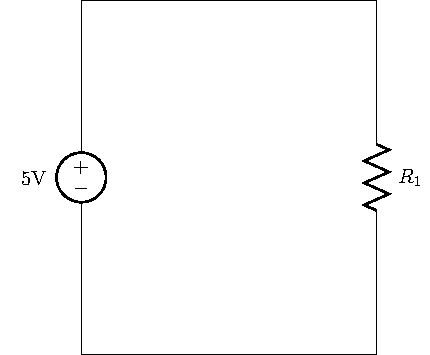
\includegraphics[width=0.4\linewidth]{../../figures/R-circuit}
Draw breadboard with resistor. Connect!
\end{center}

Describe the ideal voltage source: Will provide any current that the circuit may demand, at a perfectly constant voltage $u$. 

\subsection{Important relationsships}
\label{sec-2-4}

\subsubsection{Ohm's law}
\label{sec-2-4-1}
\(u = Ri\)

\subsubsection{Kirchoff's current law}
\label{sec-2-4-2}

\subsubsection{Kirchoff's voltage law}
\label{sec-2-4-3}

\subsection{Series connection}
\label{sec-2-5}
\begin{center}
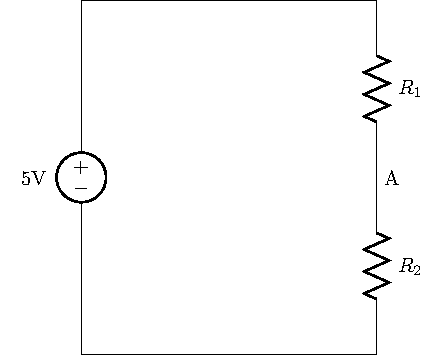
\includegraphics[width=0.4\linewidth]{../../figures/voltage-divider-circuit}
\end{center}
In the equivalent circuit with a single resistor $R_3$, then clearly $u_3=u$. And for the original circuit $u = u_1 + u_2$. The same current $i$ flows through all the elements, so from Ohm's law $u_k = R_k i_k$, we get
\( u_3 = u_1 + u_2\) and
\[ R_3 i = R_1 i + R_2 i = (R_1 + R_2) i \]
\[ R_3 = R_1 + R_2\]

This means that $i = \frac{u}{R_1 + R_2}$. So what is the voltage over $R_2$?
\[ u_2 = R_2 i = u \frac{R_2}{R_1 + R_2}. \]

\subsection{Parallel connection}
\label{sec-2-6}

\begin{center}
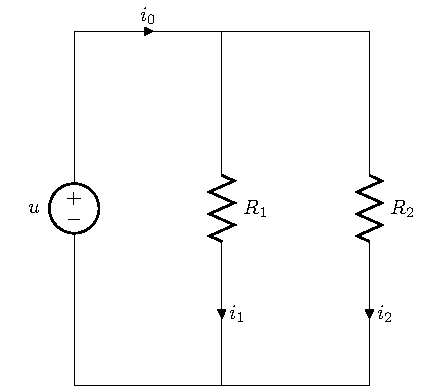
\includegraphics[width=0.4\linewidth]{../../figures/parallel-circuit}
\end{center}

In an equivalent circuit with only one resistor $R_3$, we must have \(u_3 = u = R_3 i_0\), which implies \(i_0 = \frac{u}{R_3}\).
For the two resistors in the circuit, we have \(u_1 = u = R_1 i_1\) and \(u_2 = u = R_1 i_1\), which gives \[i_1 = \frac{u}{R_1} \qquad \text{and} \qquad \(i_2 = \frac{u}{R_2}\]
From Kirchoff's current law \(i_0 = i_1 + i_2\), so  we get
\[ \frac{u}{R_3} = \frac{u}{R_1} + \frac{u}{R_2} = u \left( \frac{1}{R_1} + \frac{1}{R_2}\right)\]
hence
\[ \frac{1}{R_3} =  \frac{1}{R_1} + \frac{1}{R_2}\]
The reciprocal \(\frac{1}{R}\) of a resistance is called \emph{admittance}. 

\subsection{Safety instructions}
\label{sec-2-7}

\subsubsection{Connect everything first, then turn on the power supply}
\label{sec-2-7-1}

\subsubsection{Use low voltage, 5V}
\label{sec-2-7-2}
% Emacs 25.3.50.2 (Org mode 8.2.10)
\end{document}